\ifx\ucebnice\undefined
\documentclass[a4paper,10pt,oneside]{article}
\usepackage{latexsym}
\usepackage{amsmath}
\usepackage{amsfonts}
\usepackage{amsthm}
\usepackage{amssymb}
\usepackage{fncylab}
\usepackage{comment}
\usepackage{float}
\usepackage{wrapfig}
\usepackage{tikz}
\usepackage{tikz-qtree}
\usepackage{url}
\usepackage[bookmarks, colorlinks=false, 
            pdftitle={Úvod do programování --- Algoritmy},
            pdfauthor={Jonathan L. Verner}, 
            pdfsubject={Algoritmy a složitost}, 
            pdfkeywords={algoritmus, složitost, Python, třídění, grafy},
            bookmarksdepth=3
            ]{hyperref}
\usepackage[margin=1cm]{geometry}
\usetikzlibrary{decorations.fractals,chains,fit,shapes,patterns}
\usepackage[utf8]{inputenc}
\usepackage[T1]{fontenc}
\usepackage{attachfile}
\relpenalty=9999
\binoppenalty=9999


%----------definitions---------------------------


%math definitions

\newcommand{\R}{\mathbb R}
\newcommand{\C}{{\mathcal C}}
\newcommand{\F}{{{\mathcal F}}}
\newcommand{\U}{{{\mathcal U}}}
\newcommand{\V}{{{\mathcal V}}}
\newcommand{\cont}{{\mathfrak{c}}}
\newcommand{\force}{\Vdash}
\newcommand{\pw}{{{\mathcal P}}}
\newcommand{\MU}{{\mathbb{M}_{\mathcal{U}}}}
\newcommand{\pomega}{\pw(\omega)}


\newcommand{\src}[3]{%
\begin{program}%
\caption{#2\hfill%
\attachfile[author={Jonathan Verner},
            description={Source code for #2},
            mimetype={text/x-python},
            print=false,
            icon={Paperclip}]{kod/#1}}
\label{#3}\includecode[Python]{kod/#1}
\end{program}}


%---------numbering of the theorems------------
 \swapnumbers

 \newtheorem*{theorem*}{Theorem}
 \newtheorem{theorem}[subsection]{Theorem}
 \newtheorem{proposition}[subsection]{Proposition}
 \newtheorem{observation}[subsection]{Observation}
 \newtheorem{fact}[subsection]{Fact}
 \newtheorem{lemma}[subsection]{Lemma}
 \theoremstyle{definition}
 \newtheorem{definition}[subsection]{Definice}
 \newtheorem{question}[subsection]{Problém}
 \newtheorem{ukol}{Úloha}
 \newtheorem{cviceni}[subsection]{Cvičení}
 \newtheorem{cviceniH}[subsection]{Cvičení (*)}
 \newtheorem*{reseniIMPL*}{Řešení}
 \specialcomment{reseni}{\begin{reseniIMPL*}}{\end{reseniIMPL*}}
 \excludecomment{reseni}
 \excludecomment{todo}
 \newtheorem*{comments*}{Komentáře}
 \newtheorem*{definition*}{Definice}
 \newtheorem*{question*}{Question}
 \newtheorem{notation}[subsection]{Notation}
 \newtheorem{remark}[subsection]{Poznámka}
 \newtheorem{remark*}[subsection]{Poznámka}
 \newtheorem*{note}{Poznámka}
 \newtheorem*{ack}{Acknowledgements}
 \floatstyle{ruled}
 \newfloat{program}{htbp}{listings}[section]
 \floatname{program}{Algoritmus}
 
 \hypersetup{
    colorlinks,%
    citecolor=black,%
    filecolor=black,%
    linkcolor=black,%
    urlcolor=black
}
 
\pdfinfo{
      /Author (Jonathan Verner)
      /Title (ALG110006 Úvod do programování: Poznámky k přednášce, LS)
      /Subject (programování, algoritmy)
      /Keywords (quicksort,heapsort,dijsktra,graph,euclid)
   }
\include{pythonlisting}

\lstset{
numbers=left,
stepnumber=1,
numbersep=5pt,
numberstyle=\small\color{black}
}
%-------------opening--------------------------
\begin{document}
\title{}

% \author{Jonathan Verner}
% \address{Department of Logic, Charles University\\
% Palachovo nám. 2\\ 116 38 Praha 1, Czech Republic}
% \email{jonathan.verner{@}ff.cuni.cz}
%\thanks{The author was partially supported by }

%\subjclass[2010]{Primary }
%\keywords{}

%\begin{abstract}
%\end{abstract}
%\maketitle
\thispagestyle{empty}
\pagestyle{empty}
%\hsize=16cm
\parindent=0cm
\parskip=0.2cm

\setcounter{section}{1}
\fi
\section{Zelinář vykořisťovatel --- Halda (Heap)}

V této kapitole se budeme blíže zabývat různými způsoby, jak v paměti ukládat data a jak s nimi pracovat. Naučíme se
pracovat s frontou a zásobníkem a ukážeme si zajímavou strukturu, které se říká halda. 

\subsection*{Fronta}\pdfbookmark[2]{Fronta}{subsec:Fronta} 

Začněme následující, možná trochu šroubovanou, situací. Ve vašem městě podniká populární zelinář. Protože prodává kvalitní ovoce a zeleninu, 
které sám nakupuje od farmářů, podnikání se mu daří a jeho malou samoobsluhu navštěvuje stále více a více lidí. S tím však 
přichází i nepříjemný fenomén --- fronty. Zelinář je nadšený do moderních technologií a rozhodne se problém řešit za pomoci
elektronického zákaznického odbavovacího systému. Představuje si to takto: zákazník si naloží věci do košíku a pak si u jednoho ze stojanů,
roztroušených po obchodě, vyzvedne pořadové číslo. Se svým košíkem se pohodlně usadí do k tomu účelu přistavených
křesel a čeká, než ho zákaznický systém vyvolá. Protože zelinář počítačům příliš nerozumí, rozhodl se Vás najmout, abyste
mu naprogramovali software, který bude celý systém řídit:

\begin{question} Naprogramujte software pro zákaznický odbavovací systém.
\end{question}

Ponechme stranou technické detaily tisku čísel a podobně a soustřeďme se na jádro problému. Budeme potřebovat dvě funkce. Funkci
{\tt generujListek}, která zákazníkovi u stojanu přidělí číslo a funkci {\tt naRade}, kterou bude volat zelinář, když bude chtít
obsloužit dalšího zákazníka. V podstatě jde o to, naprogramovat takovou elektronickou frontu. To můžeme jednoduše udělat třeba
takto: budeme si prostě v nějaké proměnné, třeba {\tt last},  uchovávat poslední číslo, které jsme nějakému zákazníku přidělili a v druhé
proměnné {\tt current}, si budeme uchovávat číslo zákazníka, který je právě obsluhován. V Pythonu pak bude program vypadat třeba
takto:

\begin{python}
current=0
last=0

def generujListek():
    global last
    last = last + 1
    return last
    
def naRade():
    global last, current
    if current == last:
        return None
    else:
        current = current + 1
    return current
\end{python}

Představte si nyní, že by se požadavky trochu změnily. Čísla jsou příliš anonymní a zelinář rád lidi oslovuje jménem. Proto by chtěl,
aby uživatel do systému mohl zadat své jméno. Systém ho pak bude vyvolávat jménem. Náš výchozí program jednoduše upravíme:

\begin{python}
current=0
last=0
jmena=[]

def generujListek( jmeno ):
    global last,jmena
    last = last + 1
    jmena.append(jmeno)
    
def naRade():
    global last,jmena, current
    if current == last:
        return None
    else:
        current = current + 1
    return jmena[current-1]
\end{python}

Problém s tímto přístupem je ten, že jména se nám budou v paměti kupit a kupit a kupit $\ldots$ Po nějakém čase dojde paměť, odbavovací systém spadne a 
v obchodě se strhne mela. To je nepříjemné. Bude proto lepší program trochu přepsat. Tentokrát budeme používat pomocnou proměnnou {\tt fronta}, kde
budeme mít seznam jmen. Každého nového zákazníka přidáme na konec tohoto programu a zákazníky, které budeme odbavovat budeme naopak brát ze začátku.
Program tedy vypadá takto:

\begin{python}
fronta=[]

def generujListek( jmeno ):
    global fronta
    fronta.append(jmeno)
    
def naRade():
    global fronta
    if len(fronta) == 0:
        return None
    return fronta.pop(0)
\end{python}

Všimněte si funkce {\tt pop}, se kterou jsme se ještě nesetkali. Volání {\tt seznam.pop(n)} vrátí $n$-tý prvek seznamu {\tt seznam}
a pak ho ze seznamu smaže. Kdybychom ji chtěli sami naprogramovat, vypadala by třeba takto:

\begin{python}
def pop(seznam, index):
    ret = seznam[index]
    del seznam[index]
    return ret
\end{python}

Zkusme se nyní podívat na složitost našeho programu. V podstatě jde o to, jak jsou složité funkce {\tt append} a funkce {\tt pop}.

Jejich rychlost závisí na tom, jak Python uvnitř realizuje datový typ \emph{list}. Pythonovský \emph{list} je ve skutečnosti realizován 
jako něco, čemu se v jiných programovacích jazycích říká \emph{pole}. Když Pythonu řeknete, aby vytvořil list o 
$n$-prvcích, Python si na to v paměti vyhradí $n$ po sobě jdoucích ``chlívečků''. Když chceme přistoupit k $i$-tému prvku pole, je třeba
zjistit, kde v paměti se nachází odpovídající chlíveček. Ale to je velmi jednoduché, stačí vědět, kde pole začíná a pak k tomuto začátku přičíst
$i$-krát velikost chlívečku. Zkracování pole (funkce {\tt pop(-1), pop(0)}) je také jednoduché --- Python prostě poslední (první) ``chlíveček'' uvolní k
jinému použití. Trochu složitější je odebírání $k$-tého prvku, kde $0<k<${\tt len(pole)}. V takovém případě je třeba nejprve posunout obsah každého
chlívečku za $k$-tým o jeden chlíveček doleva --- tedy {\tt (len(pole)-k)} operací --- a pak uvolnit poslední. Nejsložitější však je prodlužování
pole, t.j. funkce {\tt append}. Pokud totiž chceme seznam zvětšit, můžou nastat komplikace. Nejjednodušší by bylo
prostě vyhradit další ``chlívečky'' za koncem pole. Jenže co když už jsou tyto chlívečky obsazeny? V takovém případě Python musí najít v paměti
někde jinde dostatek místa pro všechny chlívečky nového pole a staré pole sem překopírovat. V takové situaci tedy bude zvětšování pole mnohem náročnější.

\begin{center}
\begin{minipage}{6cm}
\lstset{
numbers=none,
stepnumber=1,
numbersep=5pt,
numberstyle=\small\color{black}
}
\begin{python}
>>> seznam = ['A','B','C',5]
>>> seznam.append('Q')
\end{python}
\end{minipage}
\begin{minipage}{5cm}
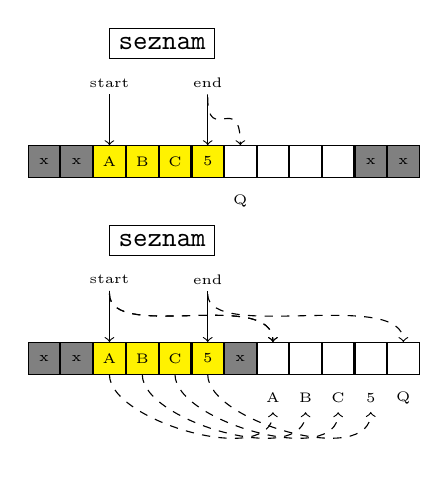
\begin{tikzpicture}
\tikzstyle{free}=[draw,minimum size=0.4cm]
\tikzstyle{used}=[draw,minimum size=0.4cm,fill=gray]
\tikzstyle{list}=[draw,minimum size=0.4cm,fill=yellow]
\begin{scope}[start chain=1 going right,node distance=0mm,shift={(5cm,2cm)}]
    \node [on chain=1,used] {\tiny x};
    \node [on chain=1,used] {\tiny x};
    \node [on chain=1,list] (startl) {\tiny A};
    \node [on chain=1,list] {\tiny B};
    \node [on chain=1,list] {\tiny C};
    \node [on chain=1,list] (endl) {\tiny 5};
    \node [on chain=1,free] (endlone){\tiny};
    \node [node distance=0.5cm,below of=endlone] {\tiny Q};
    \node [on chain=1,free] {\tiny };
    \node [on chain=1,free] {\tiny };
    \node [on chain=1,free] {\tiny };
    \node [on chain=1,used] {\tiny x};
    \node [on chain=1,used] {\tiny x};
    \node [node distance=1cm,above of=startl] (start) {\tiny start};
    \node [node distance=1cm,above of=endl] (end) {\tiny end};
    \draw[draw,->]
      (start)..controls +(south:0.1) ..(startl);
    \draw[draw,->]
      (end)..controls +(south:0.1) ..(endl);      
    \draw[dashed,->]
      (end)..controls +(south:0.8) and +(north:0.9)..(endlone);
\end{scope}
\begin{scope}[shift={(6.5cm,3.5cm)}]
    \node [draw] {\tt seznam};
\end{scope}
\begin{scope}[start chain=1 going right,node distance=0mm,shift={(5cm,-0.5cm)}]
    \node [on chain=1,used] {\tiny x};
    \node [on chain=1,used] {\tiny x};
    \node [on chain=1,list] (startl) {\tiny A};
    \node [on chain=1,list] (oldB) {\tiny B};
    \node [on chain=1,list] (oldC){\tiny C};
    \node [on chain=1,list] (endl) {\tiny 5};
    \node [on chain=1,used] {\tiny x };
    \node [on chain=1,free] (startlone){\tiny };
    \node [on chain=1,free] (B){\tiny };
    \node [on chain=1,free] (C){\tiny };
    \node [on chain=1,free] (D){\tiny };
    \node [on chain=1,free] (endlone){\tiny };
    \node [node distance=0.5cm,below of=startlone] (newA) {\tiny A};
    \node [node distance=0.5cm,below of=B] (newB){\tiny B};
    \node [node distance=0.5cm,below of=C] (newC) {\tiny C};
    \node [node distance=0.5cm,below of=D] (newD){\tiny 5};
    \node [node distance=0.5cm,below of=endlone] {\tiny Q};
    \node [node distance=1cm,above of=startl] (start) {\tiny start};
    \node [node distance=1cm,above of=endl] (end) {\tiny end};
    \node [node distance=0.5cm,below of=oldB] (copyStart) {};
    \draw[draw,->]
      (start)..controls +(south:0.1) ..(startl);
    \draw[draw,->]
      (end)..controls +(south:0.1) ..(endl);      
    \draw[dashed,->]
      (end)..controls +(south:0.8) and +(north:0.9)..(endlone);
    \draw[dashed,->]
      (start)..controls +(south:0.8) and +(north:0.9)..(startlone);
    \draw[dashed,->]
      (start)..controls +(south:0.8) and +(north:0.9)..(startlone);
    
    \draw[dashed,->]
      (startl)..controls +(south:0.8) and +(south:0.9)..(newA);      
    \draw[dashed,->]
      (oldB)..controls +(south:0.8) and +(south:0.9)..(newB);  
    \draw[dashed,->]
      (oldC)..controls +(south:0.8) and +(south:0.9)..(newC);  
    \draw[dashed,->]
      (endl)..controls +(south:0.8) and +(south:0.9)..(newD);  
      
%     \draw[draw,->]
%       (copyStart)..controls +(south:0.8) and +(south:0.9)..(newC);  
\end{scope}
\begin{scope}[shift={(6.5cm,1cm)}]
    \node [draw] {\tt seznam};
\end{scope}


\end{tikzpicture}
\end{minipage}
\end{center}


Python problémy se zvětšováním seznamů částečně obchází pomocí elegantního triku. Když totiž vytvoříte nové pole, Python si ve skutečnosti vyhradí chlívečků víc,
aby měl nějakou rezervu na zvětšování. Přidávat nové prvky je pak jednoduché do té doby, než dojde tato rezerva. Když mu rezerva dojde, musí chtě-nechtě
vyhradit místo nové a pole kopírovat. Nicméně v tuto chvíli, si opět vytvoří rezervu a pro jistotu si jí vytvoří 2-krát tak velkou jako na počátku.
Když má naopak prvek z konce pole smazat, pouze si poznačí, že pole je kratší a místo toho, aby místo na konci pole uvolnil pro jiné použití,
zvětší o něj rezervu. Ačkoliv to nemusí být jasné na první pohled, je tento postup v praxi často mnohem výhodnější. Pokud například do pole v průměru stejně 
často prvky přidáváme jako odebíráme, málokdy nám rezerva dojde a většina operací bude velmi rychlá. Tuto ``výhodnost'' lze matematicky analyzovat ---
podobně jako jsme to udělali se složitostí algoritmů --- pomocí tzv. ``amortizované složitosti'' (více viz např. \cite{Tarjan:1985}), nicméně my to nyní
dělat nebudeme a vrátíme se k našemu zelináři.

Čekat v křesle je sice pohodlnější než stát ve frontě, nicméně někteří zákazníci by si klidně připlatili, aby nemuseli čekat vůbec. Zelinář proto
za Vámi přišel s tím, abyste mu systém upravili tak, aby si lidé mohli připlatit za přednostní odbavení. Jedno možné řešení spočívá v tom, že zavedeme
fronty dvě. Frontu přednostní a frontu obyčejnou. Zákazník si při volbě čísla může připlatit, aby byl zařazen do přednostní fronty. K pokladně pak budou
vyvoláváni nejprve lidé z fronty přednostní a teprve v okamžiku, kdy je tato fronta prázdná, přijdou na řadu lidé ve frontě obyčejné. Implementace
je jednoduchá:

\begin{python}
f_obyc=[]
f_predn=[]

def generujListek( jmeno, prednostni = False ):
    global f_obyc, f_predn
    if prednostni:
        f_predn.append(jmeno)
    else:
        f_obyc.append(jmeno)
    
def naRade():
    global f_obyc, f_predn
    if len(f_predn) > 0:
        return f_predn.pop(0)
    elif len(f_obyc) > 0:
        return f_obyc.pop(0)
    else:
        return None
\end{python}

Řešení je elegantní a celkem vyhovující. Protože ale nastavená cena přednostní fronty není příliš vysoká, musí se i v ní často celkem dlouho čekat. 
Někteří movitější zákazníci by si klidně připlatili mnohem více, jen aby nemuseli čekat. Šlo by to řešit zavedením superpřednostní fronty, případně
i hyperpřednostní atd $\ldots$ Vás však napadne mnohem lepší řešení. Fronta bude jen jedna, ale při vyzvednutí lístku bude mít každý možnost zaplatit
určitou částku dle vlastní volby. Zákazníci pak budou odbavováni v pořadí podle obnosu, který zaplatili. Implementace bude tentokrát trochu
složitější:


\begin{python}
fronta = []

def generujListek( jmeno, castka ):
    global fronta
    fronta.append( [jmeno, castka] )


def naRade():
    global fronta

    # Pokud je fronta prazdna, vrat None
    if len(fronta) < 1:
      return None
      
    # Najdi zakaznika s maximalni castkou
    # (zakaznik je vzdy dvojice [ ID, castka ] )
    max_castka = zakaznici[0][1]
    max_jmeno     = zakaznici[0][0]
    max_pos    = 0
    pos        = 0
    
    for (jmeno, castka) in zakaznici:
        if castka > max_castka:
	    max_castka = castka
            max_jmeno = jmeno
            max_pos = pos
        pos = pos + 1
    
    del zakaznici[pos]
    return max_jmeno
\end{python}

Pojďme se podívat na složitost tohoto řešení. Funkce {\tt generujListek} provede pouze jednu operaci append na konec pole, tudíž má konstantní (amortizovanou)
složitost ($O(1)$), t.j. nezávisí na velikosti fronty. Funkce {\tt naRade} provede nejprve až 5 inicializačních operací (řádky 10 a 15--18)
a pak musí projít celou frontu (řádek 20) a s každým prvek provést až 2-5 operací (řádky 21--25). Má tedy v nejhorším případě složitost $5 + 5n = O(n)$,
kde $n$ je délka fronty. Vzhledem k tomu, že pro $n>1$ funkce nikdy neskončí řádkem 11, jednoduše zjistíme, že v nejlepším případě má složitost
$5 + 2n = O(n)$, tedy opět lineární v délce fronty. Ukážeme si poněkud důmyslnější řešení, které za cenu zpomalení funkce {\tt generujListek}
výrazně urychlí funkci {\tt naRade}. Trik bude spočívat v tom, že si budeme zákazníky ukládat takovým způsobem, abychom velmi rychle uměli vybrat zákazníka
s nejvyšší zaplacenou částkou. Budeme k tomu používat tzv. haldu (angl. heap), která je speciálním případem stromu. Musíme se tedy nyní chvíli zabývat stromy.

\eject
\subsection*{Stromy}\pdfbookmark[2]{Stromy}{subsec:Stromy} 

Matematický pojem stromu je dobře ilustrován následujícím obrázkem znázorňujícím dělení živých organizmů:

\begin{center}
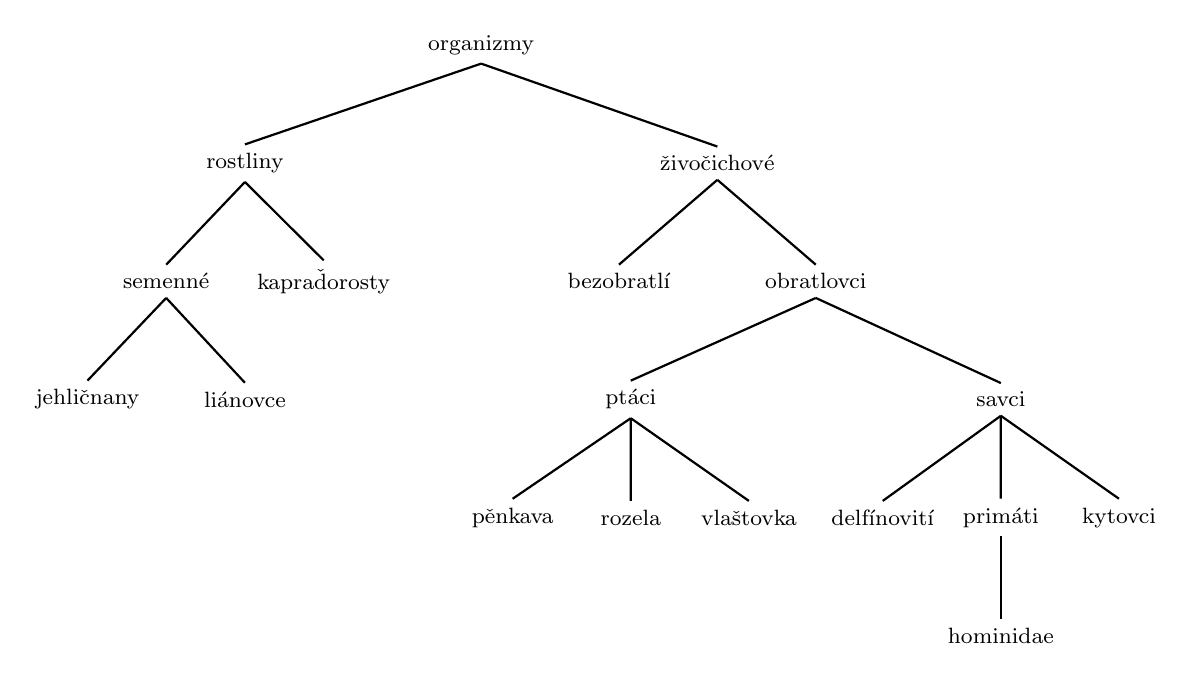
\begin{tikzpicture}
[sibling distance=6cm,-,thick]
\footnotesize
\node {organizmy}
  child {node {rostliny}
    [sibling distance=2cm]
    child {node {semenné}
      child {node {jehličnany}}
      child {node {liánovce}}
    }
    child {node {kapraďorosty}}
  }
  child {node {živočichové}
    [sibling distance=2.5cm]
    child {node {bezobratlí}}
    child {node {obratlovci}
      [sibling distance=4.7cm]
      child {node {ptáci}
        [sibling distance=1.5cm]
        child {node {pěnkava}}
        child {node {rozela}}
        child {node {vlaštovka}}
      }
      child {node {savci}
        [sibling distance=1.5cm]
        child {node {delfínovití}}
        child {node {primáti}
         [sibling distance=0.7cm]
         child {node {hominidae}}
        }
        child {node {kytovci}}
      }
    }
  };
\end{tikzpicture}
\end{center}


Schematicky ho můžeme popsat takto: na obrázku je množina kategorií (obratlovci, savci, $\ldots$), které se ve stromové terminologii často říká množina
uzlů. Mezi některými kategoriemi pak vede čára (hrana), znázorňující vztah kategorie-podkategorie (obratlovci--savci, $\ldots$), ve stromové terminologii se tomuto vztahu 
často říká vztah rodič--dítě (motivace pochází z rodokmenů, které se také často znázorňují pomocí stromů). Zavedeme si ještě několik pomocných pojmů:

\begin{definition}
\emph{kořen} je uzel, který je úplně na vrcholu, t.j. čáry vedou pouze z něj, žádná čára nevede do něj. Na našem obrázku je kořenem kategorie ``organizmy''.
Naopak \emph{list} je uzel, ze kterého nevede žádná čára (např. ``vlaštovka'', ...) a uzly, které nejsou listy (včetně kořene) budeme souhrnně nazývat
\emph{vnitřními} uzly. Pokud má uzel alespoň dvě děti (t.j. vedou z něj dvě čáry), řekneme, že se \emph{větví}, resp. že je to \emph{větvící} uzel.
Pokud mají všechny uzly mimo listů dvě děti, říkáme, že strom je binární (podobně definujeme ternární strom atd.). \emph{Cestou} ve stromu rozumíme posloupnost uzlů, 
které jsou postupně mezi sebou pospojované hranami vedoucími vždy od rodiče k dítěti. Cestu od kořene k nějakému 
listu nazveme \emph{větví}. \emph{Hloubkou} stromu rozumíme délku nejdelší větve. \emph{Hladinou} ve stromě rozumíme množinu uzlů, které mají stejnou hloubku.
Uzel A je \emph{potomkem} uzlu B, pokud z B do A vede cesta. V takovém případě říkáme též, že uzel B je \emph{předkem} uzlu A. 
\end{definition}

\begin{note}\footnotesize
Formálně lze tuto situaci modelovat různými způsoby. Například v teorii množin je strom definován jako částečně uspořádaná množina $(T,\leq)$,
kde prvky $t\in T$ odpovídají uzlům a pro každý uzel $t\in T$ je uspořádání $\leq$ zúžené na množinu $\{s\in T:s\leq t\}$ jeho předchůdců dobré.
Jiný způsob, který pro nás bude důležitější, reprezentuje strom jako speciální případ tzv. grafu. Ke grafům se dostaneme později ve větší podrobnosti.
\end{note}

Pojďme se nyní podívat, jak je možné tuto situaci reprezentovat v Pythonu. Bude pro nás důležité, že v každém uzlu
chceme uchovávat nějaká data --- třeba pojmenování toho uzlu. Nejjednodušší bude reprezentovat uzel jako dvojici  {\tt u = (data, deti)}, 
kde {\tt deti} je seznam uzlů, které jsou dětmi uzlu {\tt u}. Zde je názorný příklad:

\begin{center}
\begin{minipage}{8cm}
\lstset{
numbers=none,
stepnumber=1,
numbersep=5pt,
numberstyle=\small\color{black}
}
\begin{python}
>>> T = ('Koren',[
	          ('List A',[]),
		  ('B',[
			('List C',[]),
			('List D',[])
			])
		  ])
\end{python}
\end{minipage}
\begin{minipage}{5cm}
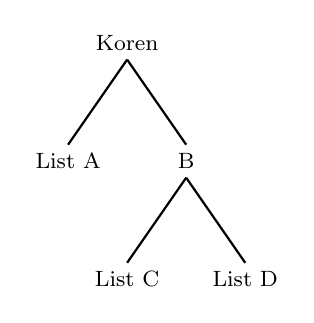
\begin{tikzpicture}
[sibling distance=1.5cm,-,thick]
\footnotesize
\node {Koren}
  child {node {List A}}
  child {node {B}
    [sibling distance=1.5cm]
    child {node {List C}}
    child {node {List D}}
  };
\end{tikzpicture}
\end{minipage}
\end{center}

Ukažme si na dvou jednoduchých příkladech, jak s takovými stromy pracovat. Často bude velmi přirozené používat rekurzi. Například procedura, 
která vrátí seznam jmen všech listů může vypadat takto:

\begin{python}
def listy(T):
  ret = []
  if len(T[1]) == 0:
    # T je list (nemá žádné děti), vrátíme jméno T
    return [T[0]]
  else:
    # Projdeme všechny děti a do našeho seznamu přidáme listy,
    # které jsou jejich potomkem 
    for t in T[1]:
      ret = ret + listy(t)
  return ret
\end{python}

Zkusme si nyní nějaký strom vytvořit. Budeme chtít naprogramovat funkci, která dostane jako parametr číslo a vytvoří následující strom. V každém uzlu
stromu bude uloženo nějaké číslo, v kořeni bude uloženo číslo dané vstupním parametrem. Děti každého uzlu budou odpovídat všem dělitelům $>1$, listy
tedy budou odpovídat prvočíselným dělitelům. Například pro číslo dvacet budeme chtí vytvořit následující strom:
\begin{center}
\begin{tikzpicture}
\node { 20 }
   child {    node { 2 }
   }
   child {    node { 4 }
     child {      node { 2 }
     }
   }
   child {    node { 5 }
   }
   child {    node { 10 }
     child {      node { 2 }
     }
     child {      node { 5 }
     }
   };
\end{tikzpicture}
\end{center}

V Pythonu může naše funkce vypadat třeba takto:

\begin{python}
def delitele(n):
  ret = []
  for d in range(2,n/2+1):
    if n % d == 0:
      ret.append(d)
  return ret
  
def strom_delitelu(n):
  delit = delitele(n):
  deti = []
  for d in delit:
    deti.append(strom_delitelu(d))
  return (n,deti)
\end{python}

\subsection*{Haldy}\pdfbookmark[2]{Haldy}{subsec:Haldy} 

Vraťme se nyní k našemu zelináři. Řekli jsme, že budeme chtít ukládat zákazníky tak, abychom uměli velmi rychle vybírat zákazníka
s nejvyšší zaplacenou částkou a podobně rychle zákazníky i přidávat. Řešení spočívá v tom, že je budeme ukládat do stromové struktury,
které se říká halda. Halda je speciální případ binárního stromu, ve kterém je v každém uzlu mimo ostatních dat ještě navíc uloženo
nějaké číslo. Jakožto strom je to strom, ve kterém se každý uzel, který není listem, větví a všechny listy jsou na poslední nebo 
předposlední hladině s tím, že listy na poslední hladině jsou ``co nejvíce vlevo''. Navíc pro každý uzel platí, že číslo, které je v něm uloženo,
že je menší než čísla uložená ve všech jeho potomcích. Příkladem haldy je například následující strom:
\begin{center}
\Tree [.2 [.10 [.11 ] [.10 ] ] [.20 ] ]
\end{center}

Naopak ani jeden z následujících stromů haldou není.
\begin{center}
(A)
\begin{minipage}{4cm}
\Tree [.0 [.10 [.11 ] [.9 ] ] [.20 ] ] 
\end{minipage}
(B)
\begin{minipage}{6cm}
\Tree [.0 [.10 [.11 [.15 ] [.16 ] ] [.9 ] ] [.20 [.30 [.35 ] [.37 ] ] [.31 [.32 ] [.33 ] ] ] ]
\end{minipage}
(C)
\begin{minipage}{4cm}
\Tree [.0 [.10 [.11 ] [.9 ] ] ]
\end{minipage}
\end{center}
Ve stromu (A) je porušena podmína, že uzly jsou menší než jejich potomci ($10\not\leq 9$), ve stromu (B) je
porušena podmínka, že listy na poslední hladině mají být úplně vlevo a ve stromu (C) je porušena podmínka,
že každý uzel, který není listem, se musí větvit.

Prvky se do haldy přidávají tak, že se vytvoří nový list a do něj se prvek vloží. Tím může dojít k porušení
podmínky, že uzly jsou menší než potomci. Proto musíme zkontrolovat, zda je vložený prvek větší než jeho rodič.
Pokud není, s rodičem ho vyměníme a musíme dále zkontrolovat rodiče s jeho rodičem. Pokud je vše O.K., skončíme,
jinak pokračujeme v prohazovaní dokud se nedostaneme do kořene, který žádného rodiče nemá.

Příklad přidávání prvku $1$ do haldy:

\begin{center}
\begin{minipage}{4cm}
\Tree [.2 [.10 [.11 ] [.10 ] ] [.20 ] ]
\end{minipage}
$\Rightarrow$
\begin{minipage}{4cm}
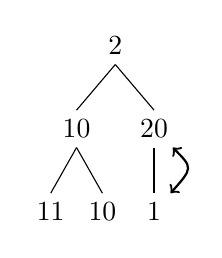
\begin{tikzpicture}
\Tree [.2 [.10 [.11 ] [.10 ] ] [.\node(a){20}; [.\node(b){1}; ] ] ]
\draw[thick,<->](a)..controls +(south east:0.7).. (b);
\end{tikzpicture}
\end{minipage}
$\Rightarrow$
\begin{minipage}{4cm}
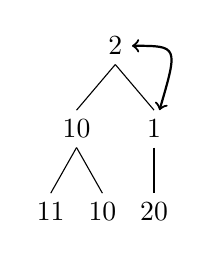
\begin{tikzpicture}
\Tree [.\node(a){2}; [.10 [.11 ] [.10 ] ] [.\node(b){1}; [.20 ] ] ]
\draw[thick,<->](a)..controls +(east:0.8).. (b);
\end{tikzpicture}
\end{minipage}
$\Rightarrow$
\begin{minipage}{4cm}
\Tree [.1 [.10 [.11 ] [.10 ] ] [.2 [.20 ] ] ]
\end{minipage}
\end{center}

Naopak z hlady se (vrchní) prvek odebírá tak, že se vrátí hodnota v kořeni a nahradí se hodnotou v nejpravějším
listu na poslední hladině a tento list se smaže. Tím může být opět porušeno pravidlo, že uzly jsou menší než následníci, proto musíme zkontrolovat, zda
nová hodnota kořene je větší než hodnota obou jeho dětí. Pokud není, vyměníme tuto hodnotu s hodnotou menšího
dítěte a pokračujeme v kontrolování tohoto dítěte dokud není vše O.K., nebo dokud se nedostaneme do listu, kde
je vše O.K. z definice.

\begin{center}
\begin{minipage}{4cm}
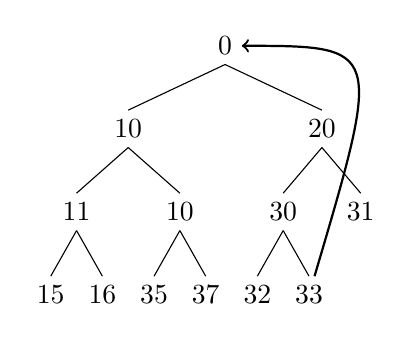
\begin{tikzpicture}
\Tree [.\node(a){0}; [.10 [.11 [.15 ] [.16 ] ] [.10 [.35 ] [.37 ] ] ] [.20 [.30 [.32 ] [.\node(b){33}; ] ] [.31 ] ] ]
\draw[thick,<-](a)..controls +(east:2).. (b);
\end{tikzpicture}
\end{minipage}
$\Rightarrow$
\begin{minipage}{4cm}
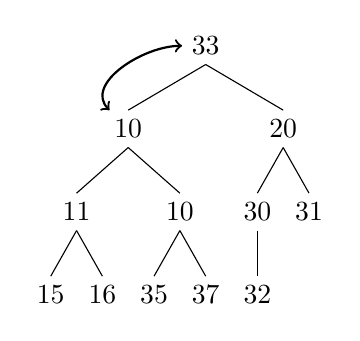
\begin{tikzpicture}
\Tree [.\node(a){33}; [.\node(b){10}; [.11 [.15 ] [.16 ] ] [.10 [.35 ] [.37 ] ] ] [.20 [.30 [.32 ] ] [.31 ] ] ]
\draw[thick,<->](a)..controls +(west:0.8) and +(north west:0.8) .. (b);
\end{tikzpicture}
\end{minipage}
$\Rightarrow$
\begin{minipage}{4cm}
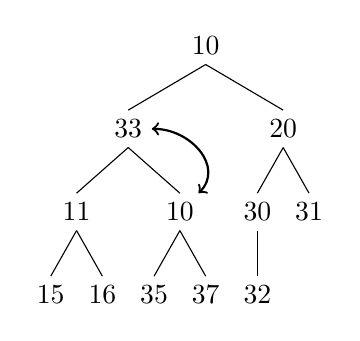
\begin{tikzpicture}
\Tree [.10 [.\node(a){33}; [.11 [.15 ] [.16 ] ] [.\node(b){10}; [.35 ] [.37 ] ] ] [.20 [.30 [.32 ] ] [.31 ] ] ]
\draw[thick,<->](a)..controls +(east:0.8) and +(north east:0.8) .. (b);
\end{tikzpicture}
\end{minipage}
$\Rightarrow$
\begin{minipage}{4cm}
\Tree [.10 [.10 [.11 [.15 ] [.16 ] ] [.33 [.35 ] [.37 ] ] ] [.20 [.30 [.32 ] ] [.31 ] ] ]
\end{minipage}
\end{center}

Jaká je složitost těchto operací? Pro přidávání potřebuji
\begin{itemize}
 \item přidat prvek na konec haldy
 \item a v nejhorším případě projít stromem od listu ke kořeni a v každém kroku provést jedno porovnání a jednu výměnu
\end{itemize}

Složitost přidání v nejhorším případě tedy bude záviset na výšce stromu. Není těžké si uvědomit, že pokud je strom haldou a má $n$
uzlů, pak jeho výška bude buď $\log_2 n$ nebo,  $\log_2 n + 1$. Celková složitost tedy bude asymptoticky $O(\log n)$ + složitost
přidání prvku na konec haldy. To bude samozřejmě záviset na konkrétním naprogramování, ale v jakékoliv rozumné verzi to nebude
horší než $O(\log n)$. Podobně to vyjde pro operaci odebrání prvku. Pokud bychom chtěli jen zjistit, jaký je nejmenší prvek,
bude to dokonce $O(1)$. 

Zavedli jsme haldu takovým způsobem, aby měla v kořeni nejmenší číslo. Pro náš zelinářský software by se však 
hodilo naopak mít v kořeni číslo největší. Rozmyslete si, že pokud v haldě obrátím podmínku na čísla, t.j. pokud budu požadovat,
aby číslo uzlu bylo větší, než číslo všech jeho potomků, bude všechno opět fungovat (po jednoduché úpravě operací). V následující
praktické implementaci v Pythonu uvedeme tuto ``opačnou'' verzi haldy.

Ukážeme si nyní práci s haldou v Pythonu. Mohli bychom s ní pracovat jako s obyčejným stromem. V takovém případě by bylo dobré si u každého
uzlu navíc pamatovat i jeho rodiče. Tedy uzel by mohl být třeba čtveřice {\tt (data, hodnota, rodic, deti)}. S takovouto reprezentací
by se ale pracovalo trochu nešikovně, protože neumožňuje jednoduše zjistit nejlevější list na předposlední hladině (resp. na poslední, pokud takový není).
Bude proto lepší si umět haldu uchovávat v seznamu (a v budoucnu se nám to bude hodit). 

\begin{todo}
Obecně lze v poli ukládat i jiné stromy resp. grafy než haldu --- a naše původní reprezentace je ve skutečnosti (uvnitř Pythonu)
právě taková.
\end{todo}

Haldu budeme ukládat po jednotlivých hladinách, každý prvek seznamu bude dvojice {\tt (data, hodnota)}. Jeho index v poli bude určovat jeho pozici ve stromu. 
Na prvním místě bude kořen, na druhém a třetím jeho případné dvě děti, a tak dále. Protože ukládaný strom je haldou, můžeme si z pozice uzlu {\tt u} jednoduše vypočítat
pozice jeho dětí a rodičů. Je-li totiž jeho pozice {\tt n}, pak jeho děti mají pozici {\tt 2*n + 1} a {\tt 2n + 2} a jeho rodič má index
{\tt (n-1)/2}. Uvědomte si, že zde využíváme faktu, že jde o haldu, u obecného stromu by to nefungovalo! Elegance tohoto přístupu spočívá v tom, 
že nejlevější list je prostě poslední prvek pole. Operace v Pythonu pak můžou vypadat třeba následovně jako na výpisu \ref{alg:heap}.

\src{heap}{Operace s haldou}


\subsection*{Zelinář --- pokračování}\pdfbookmark[2]{Zelinář --- pokračování}{subsec:zelinarcont} 

Říkali jsme, že upravíme náš zákaznický systém tak, aby jak tištění lístků (funkce {\tt generujListek}) tak vyvolávání zákazníků
(funkce {\tt naRade}) pracovaly rychle. Uděláme to tak, že využijeme výše uvedené funkce pro práci s haldou a zákazníky si budeme
ukládat do haldy. Funkce budou tedy vypadat takto:

\begin{python}
halda = []
def generujListek( jmeno, castka ):
  push( halda, jmeno, castka)

def naRade():
  return pop( halda ) 
\end{python}

\begin{cviceni} Náš kamarád zelinář si upravený zákaznický systém velmi pochvaluje, nicméně všiml si jedné nepříjemné vlastnosti.
Občas se totiž stane, že nějaký šetřivý zákazník zaplatí za odbavení malou částku a pak se nikdy nedostane na řadu, protože ho
všichni ostatní přeplatí. A tak se mu v obchodě hromadí neodbavení šetřiví zákazníci $\ldots$ Požádal Vás proto, abyste systém
upravili tak, aby bral v potaz nejen zaplacenou částku, ale i čas strávený čekáním. Na Vás teď je navrhnout úpravu. Když se nad
tím zamyslíte, nebude to vůbec složité $\ldots$
\end{cviceni}

\begin{reseni}
Stačí si pamatovat celkový počet odbavených zákazníků a při odbavování tento počet (případně vynásobený nějakou vhodnou konstantou)
odečíst od zaplacené částky. 
\end{reseni}

\ifx\ucebnice\undefined
\renewcommand{\refname}{\textbf{Literatura}}
\bibliographystyle{mujstyl}
\bibliography{ref}

\end{document}
\fi